\documentclass[12pt,twoside,letterpaper]{report}
\usepackage{graphicx}
\usepackage{listings}
\setlength\topmargin{0in}
\setlength\headheight{0in}
\setlength\headsep{0in}
\setlength\textheight{9.0in}
\setlength\textwidth{6.5in}
\setlength\oddsidemargin{0in}
\setlength\evensidemargin{0in}
\setlength{\parskip}{12pt}
\pagestyle{plain}
\raggedright
\title{mTrader Visual Inspection}
\author{Cameron Lowell Palmer}
\date{September 2010}

\begin{document}
\maketitle

\section*{Start and Stop}
Locking the phone should cause the application to logout. Upon unlocking the phone the device should automatically reconnect and update.

\section*{Network Change}
Switching networks, Edge, 3G, WiFi, should result in an automatic reconnect and the application should continue streaming.

\section*{My List Tab}
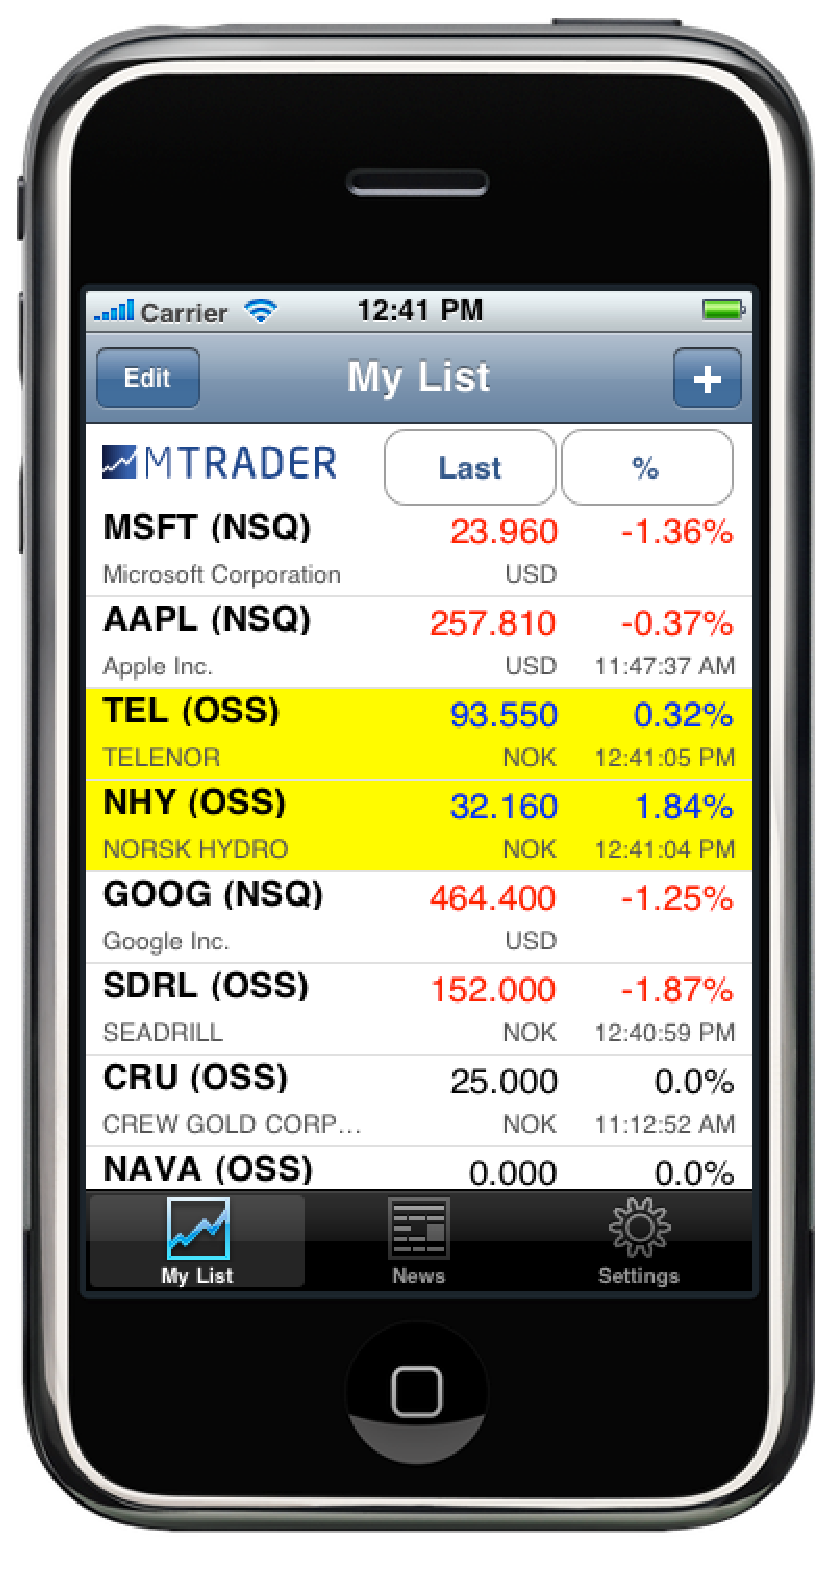
\includegraphics[scale=0.5]{myList}

\subsection*{Loading}
Each load of the program should maintain the same ordering and if loaded from TOT the order should be respected in mTrader.

\subsection*{Running}
Each cell should have the following:

\begin{tabular}{ l l l }
\hline
TICKER (EXCHANGE) & Last & Percent Change \\
Full Name & Currency & Time of last trade \\
\hline
\end{tabular}

Negative prices are red, positive blue. The whole second line gray. The line should flash when an up or down trade occurs.

Buttons should cycle through Last, Bid, Ask and Percent, Up/Down, Last respectively and update the values in the column.

\subsection*{Adding Instrument}
New instruments should be added to the bottom of the list and the list should be scrolled there.

\subsection*{Deleting Instrument}
Either swiping the row from left to write or tapping edit should allow you to successfully delete and instrument and it should not return upon quitting and restarting the app.

\section*{Symbol Search}

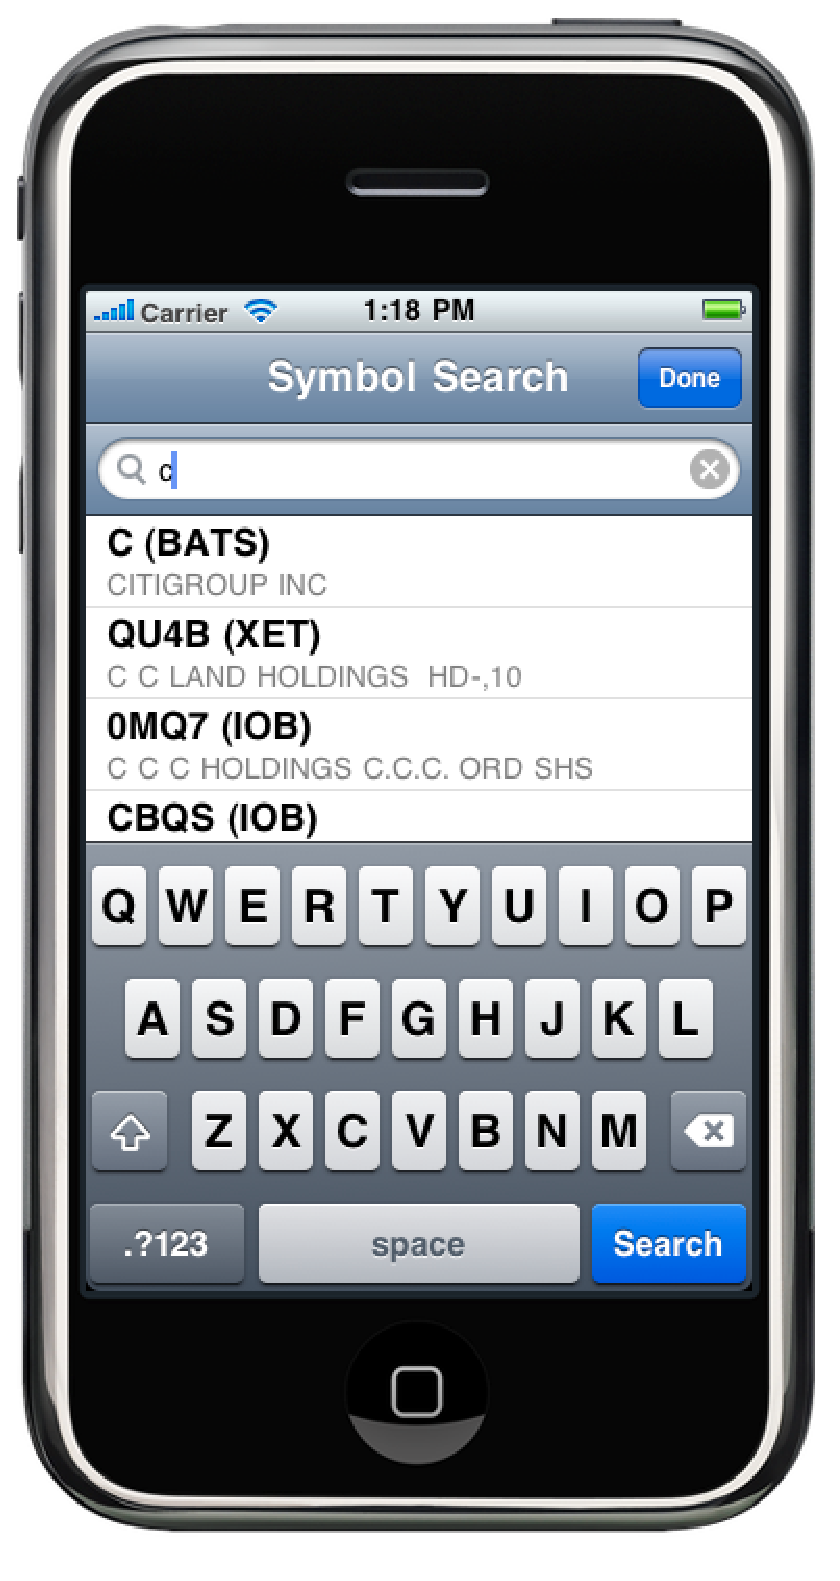
\includegraphics[scale=0.5]{symbolSearch}

Typing should result in a dynamic list being presented with instruments. Tapping in that window should cause the keyboard to disappear and then adding instruments is a matter of tapping them and watching them disappear. You should not see instruments you have already added, and you should not ever see a couldn't add an instrument dialog. If you see a unable to add instrument there is a problem with the symbol list on the server or the server itself.

Clearing the search dialog should remove all results, typing a non-matching character should also clear the results.

Tapping Done causes the Symbol Search dialog to disappear.

\section*{Symbol Detail}

In the top-left box should appear Last price, Change, Percent change, Time of last trade, and a line graph representing intraday activity.

In the top-right box Open, High, Low, VWAP, Volume, Trades, Turnover, B Lot, B Lot Volume, Avg Volume, and Avg Value.

Tapping the intraday chart should launch the graph modal view. The back button takes you back to My List.

\subsection*{Graph Modal}
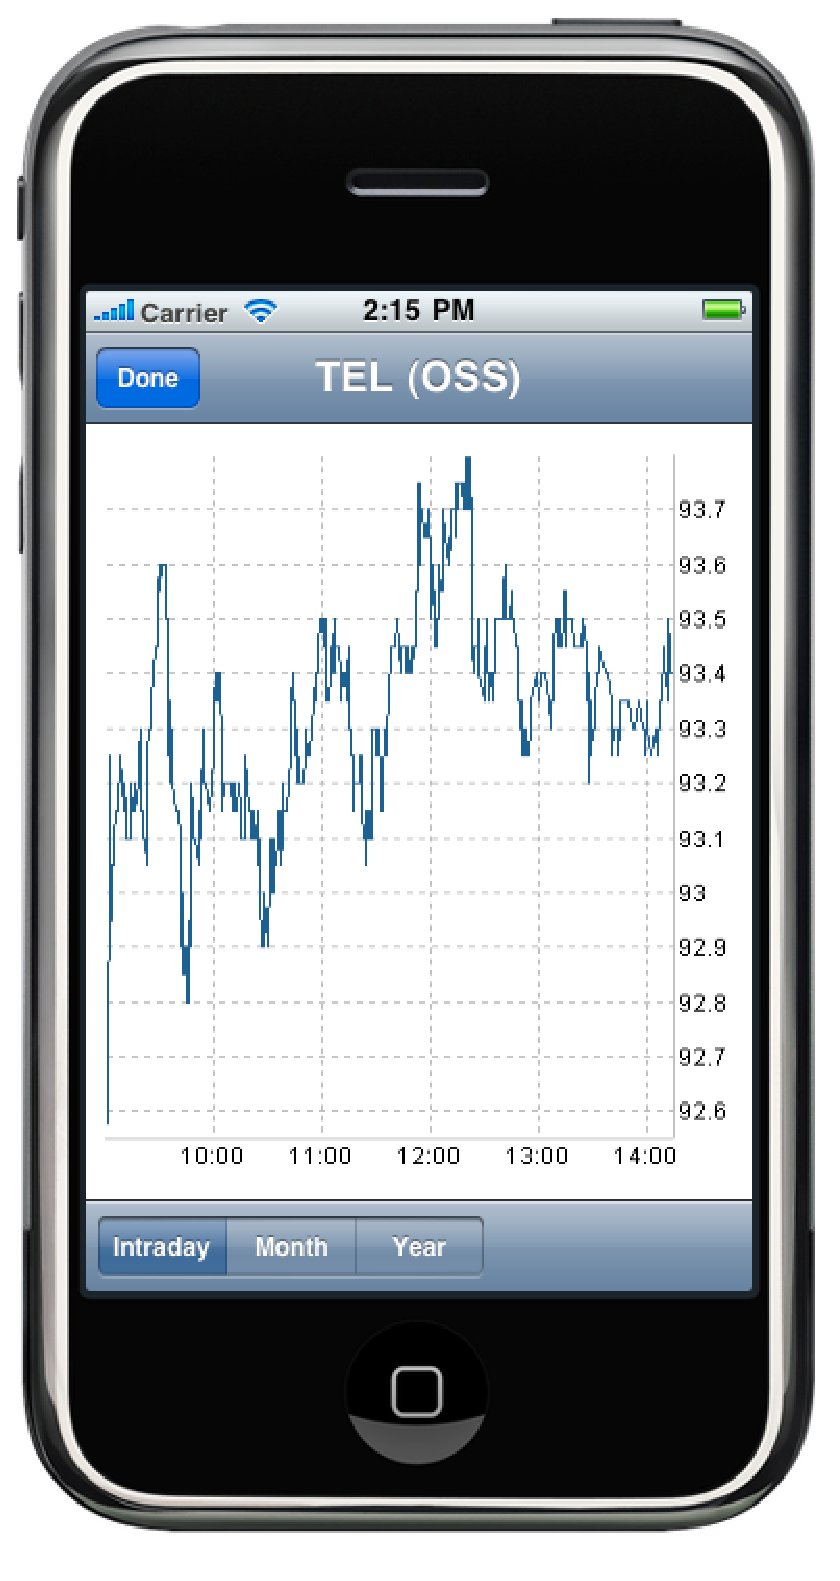
\includegraphics[scale=0.5]{symbolDetailGraphModal}

The graph modal should have reasonable version of the Intraday, Month, Year for that symbol. The image should be reasonably sharp.

\subsection*{Orderbook}
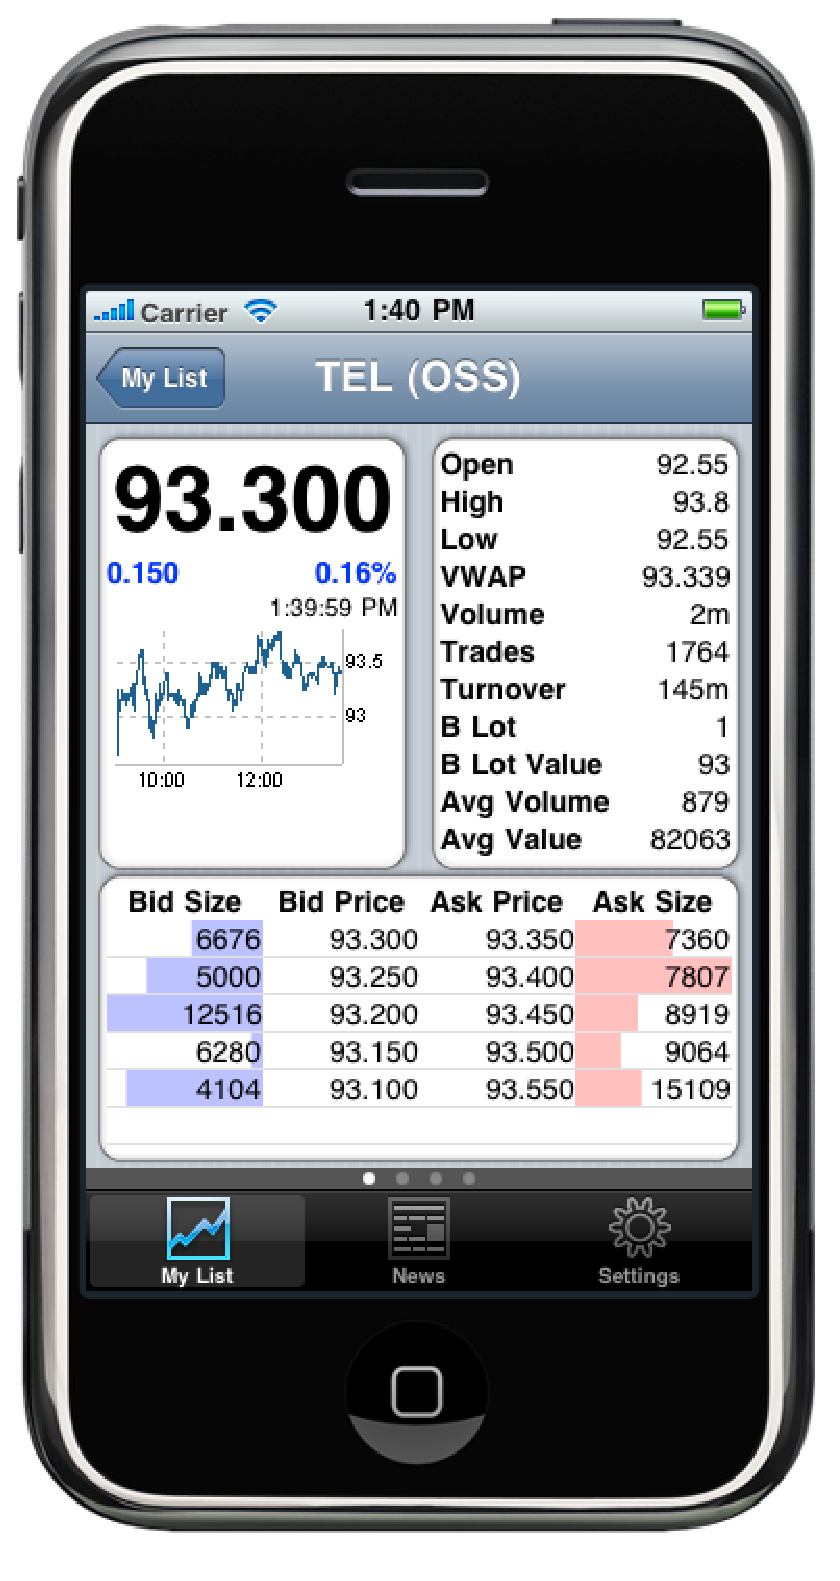
\includegraphics[scale=0.5]{symbolDetailOrderbook}

The Orderbook should have this format:
\begin{tabular}{ l l l l }
\hline
Bid Size & Bid Price & Ask Price & Ask Size \\
\hline
\end{tabular}

The bars should be blue for bid size and red for ask size. The Bid Prices should be unique values that go from highest to lowest, and Ask Prices should be unique values that go from lowest to highest. The relative sizes of bars should match the relationship in the bid and ask sizes. Please, check to make sure this relationship is true over a minute or two of trades. The image provided has bars that don't make sense with the volume sizes.

Tapping the orderbook should launch a modal version of the identical view.

If the symbol doesn't have an orderbook it should display 'No Orderbook Available' or if the item is a fund or index the orderbook view should not appear at all.

\subsection*{Historic Trades}
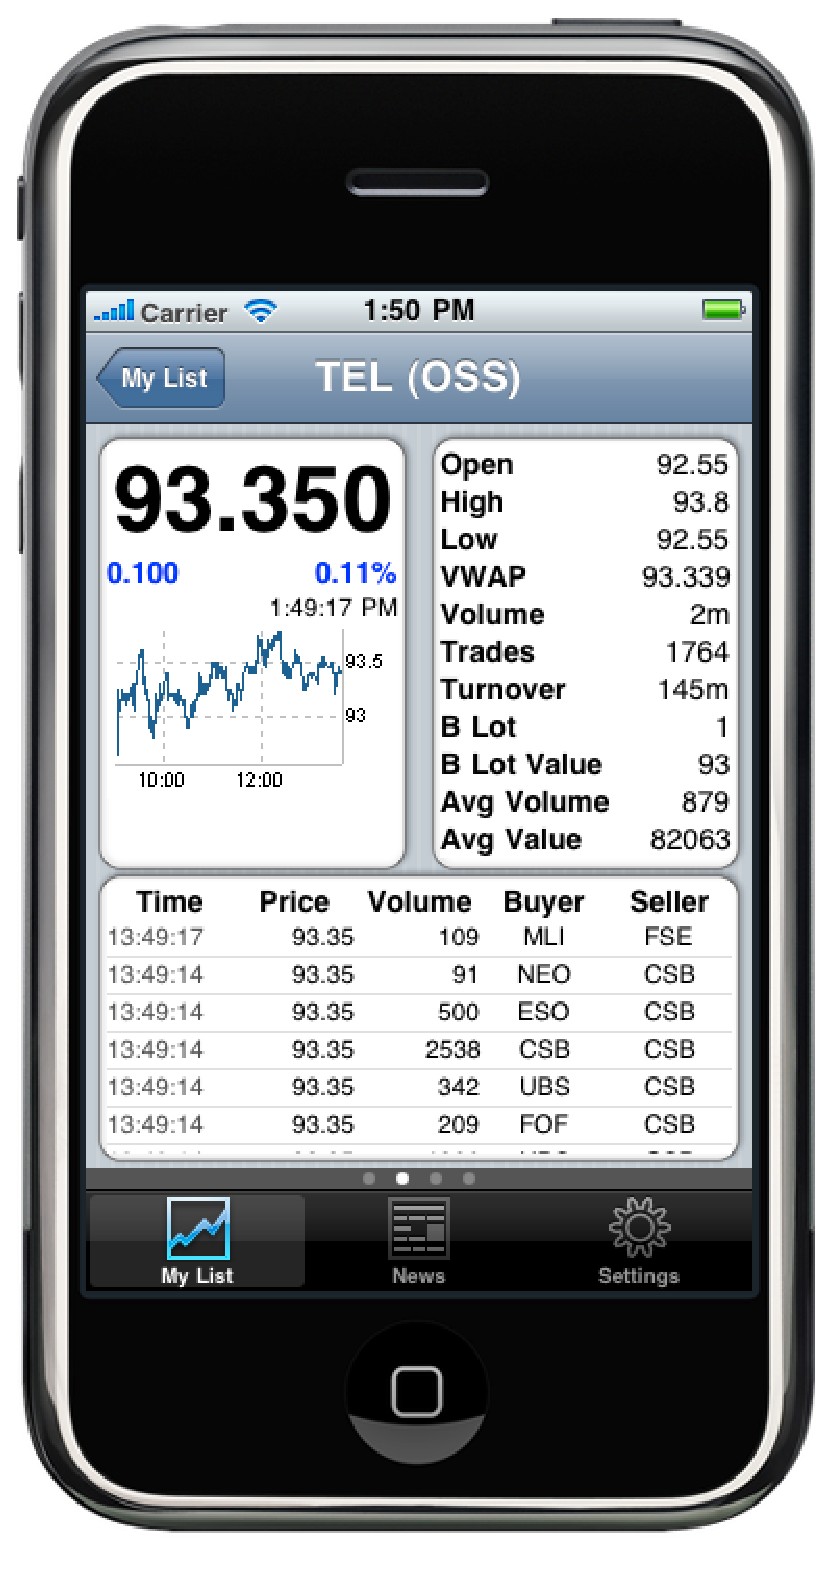
\includegraphics[scale=0.5]{symbolDetailHistoricTrades}

The Historic Trades should have this format:
\begin{tabular}{ l l l l l }
\hline
Time & Price & Volume & Buyer & Seller \\
\hline
\end{tabular}

The times of trades should descend from newest to oldest today with the relevant values displayed in the other column.

Tapping the historic trades window should launch a modal version of the identical view with more rows that can be scrolled through.

\subsection*{News}
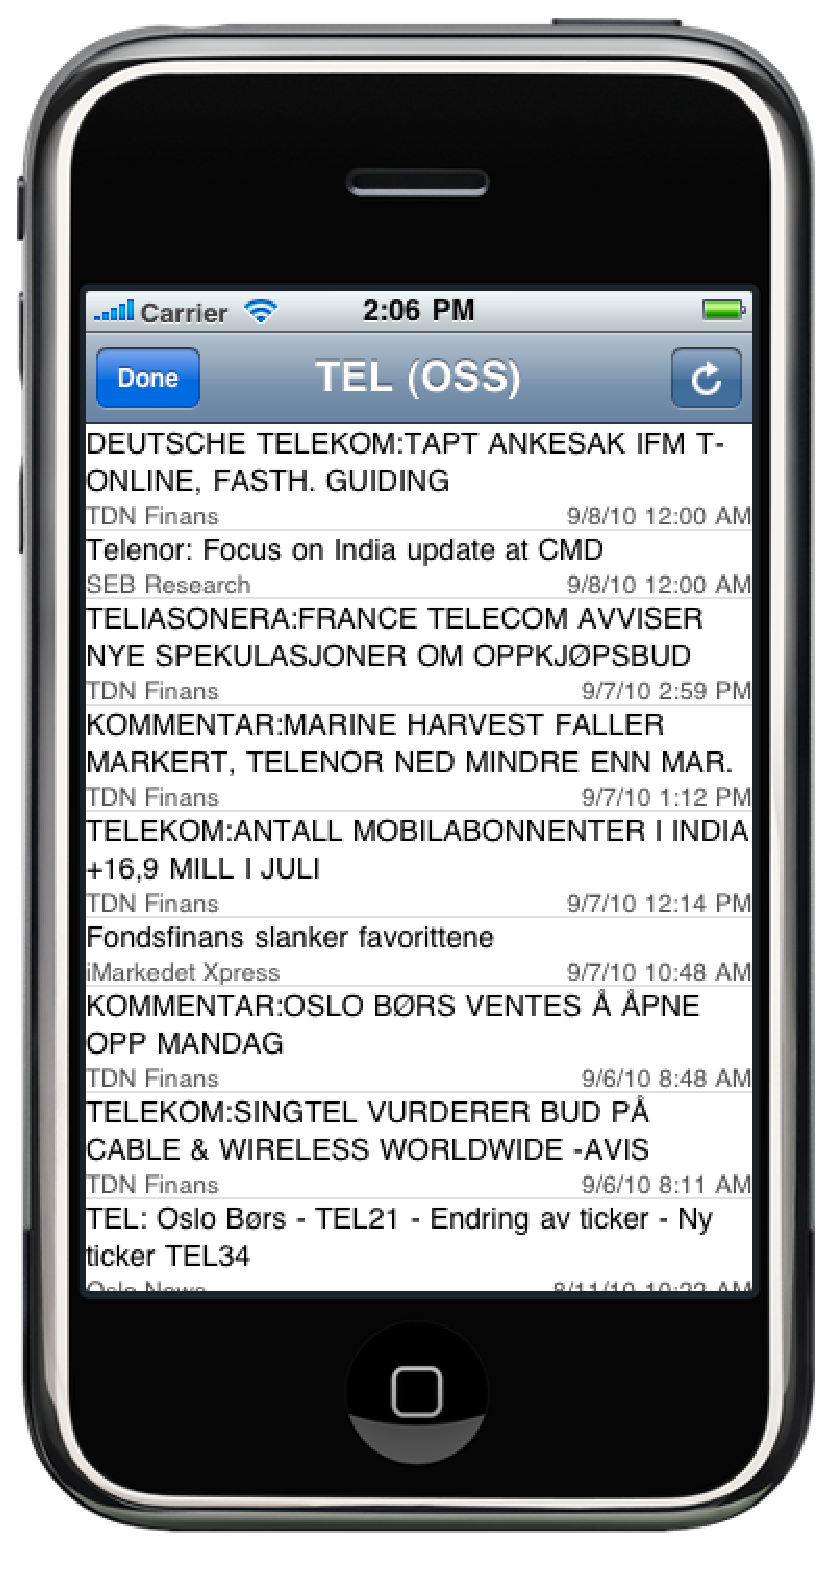
\includegraphics[scale=0.5]{symbolDetailNewsHeadings}

Symbol News is only interesting in its modal form but the symbol news box should show the same first articles as the modal version.

Flash news articles are Red and should have no text, all other articles should contain text when tapped. Please check the date/time on the right hand side. They should go from newest to oldest. The lower left side of each row should contain the news feed that provided the article. All the articles should reference the current symbol, and if there are duplicates of the same article they should be in different news feeds or a Flash and a Full article.

Tapping Refresh should update the news to display new articles

\subsection*{Other Information}
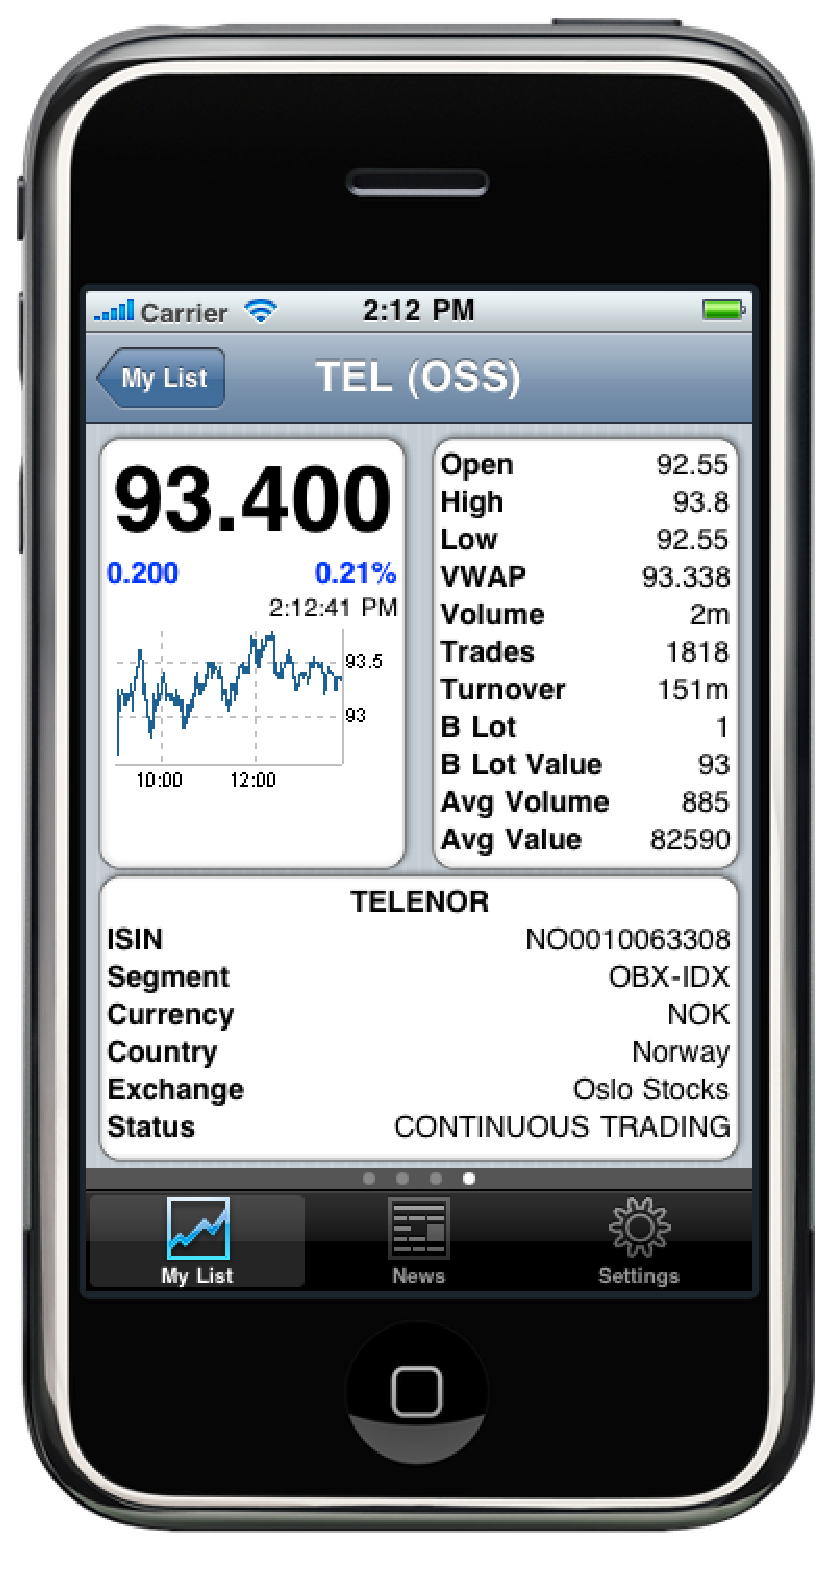
\includegraphics[scale=0.5]{symbolDetailOtherInformation}

This simply contains Full name of symbol, ISIN, Segment, Currency, Country, Exchange, Status

Tapping does nothing.

\section*{News Tab}
\subsection*{Articles}
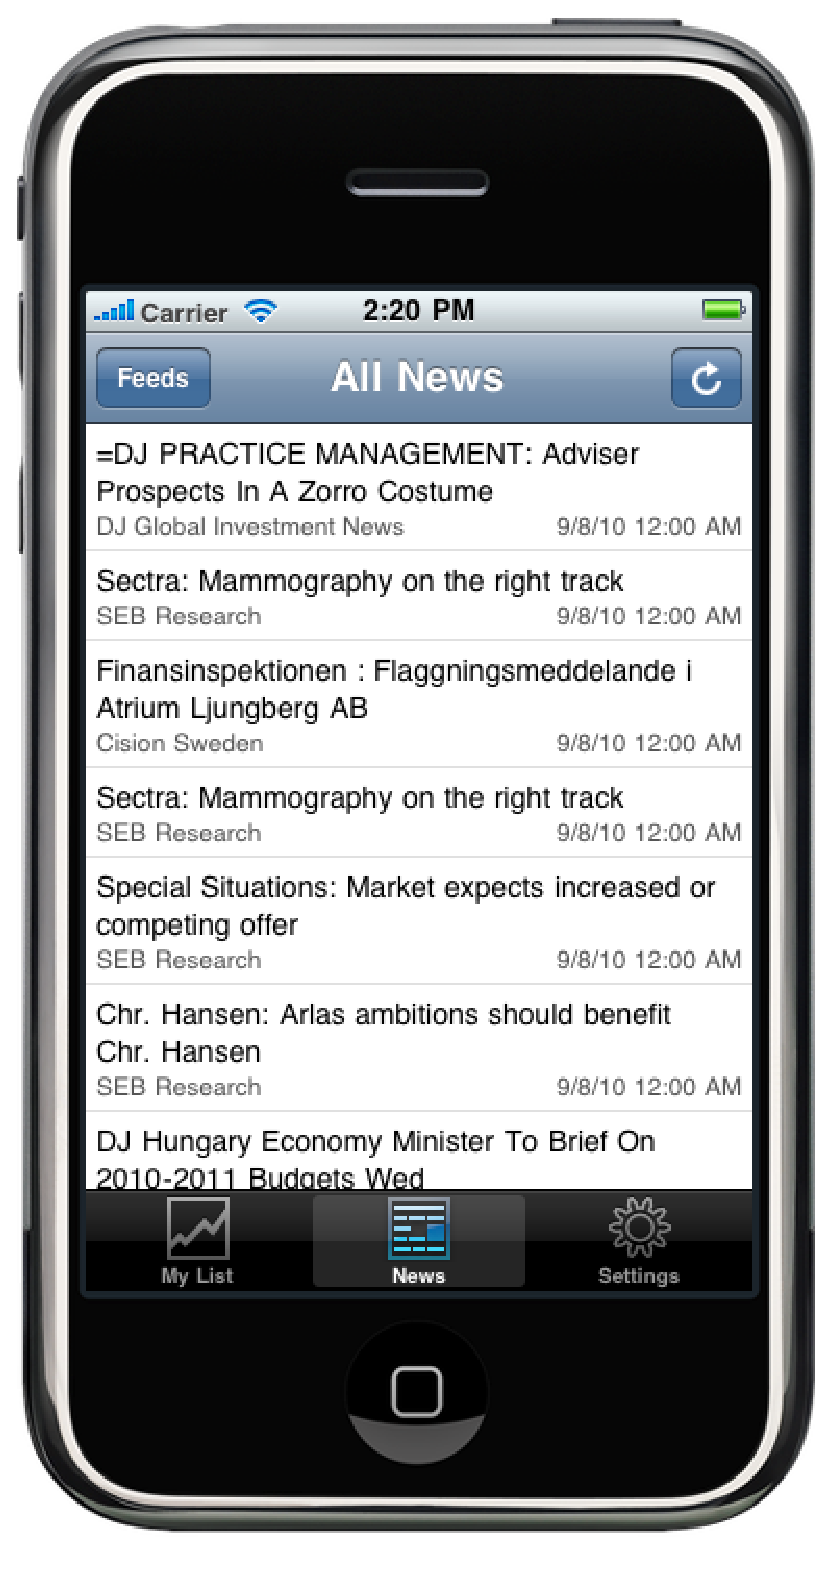
\includegraphics[scale=0.5]{newsArticles}

The News articles should display newest to oldest and the Feed selection should match up with the articles presented.

Tapping refresh should download news articles and is most obvious under Feeds like the Dow Jones International.

Selecting an article slides in a news article.

\subsection*{News Article}
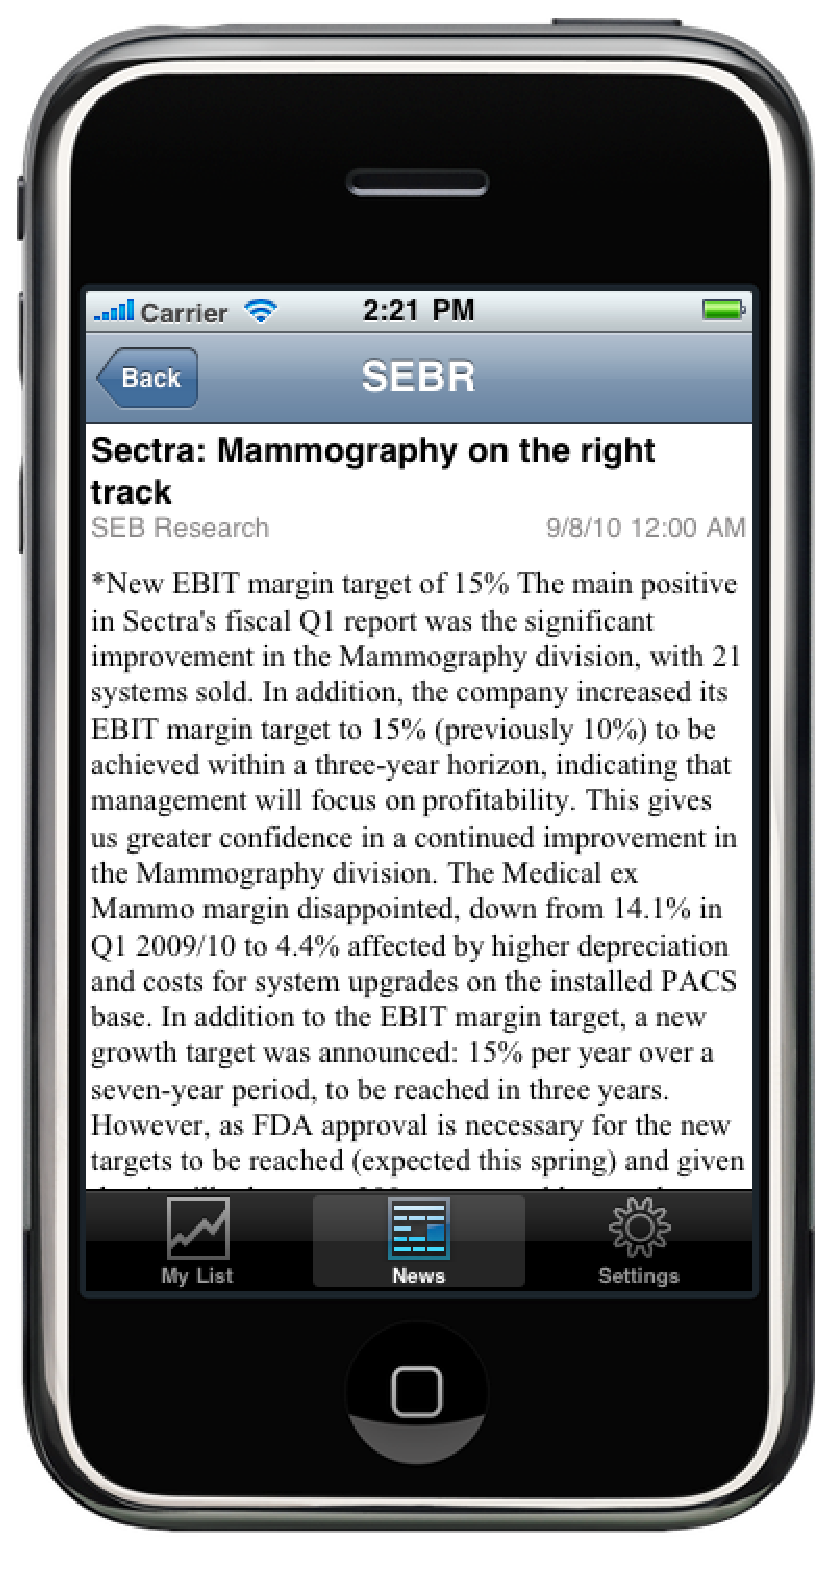
\includegraphics[scale=0.5]{newsArticle}

The news article should wrap nicely be zoomable, Copy/Paste works, hyperlinks should work and launch Safari, and the header should match up with the information on the previous page.

\subsection*{News Feed Selection}
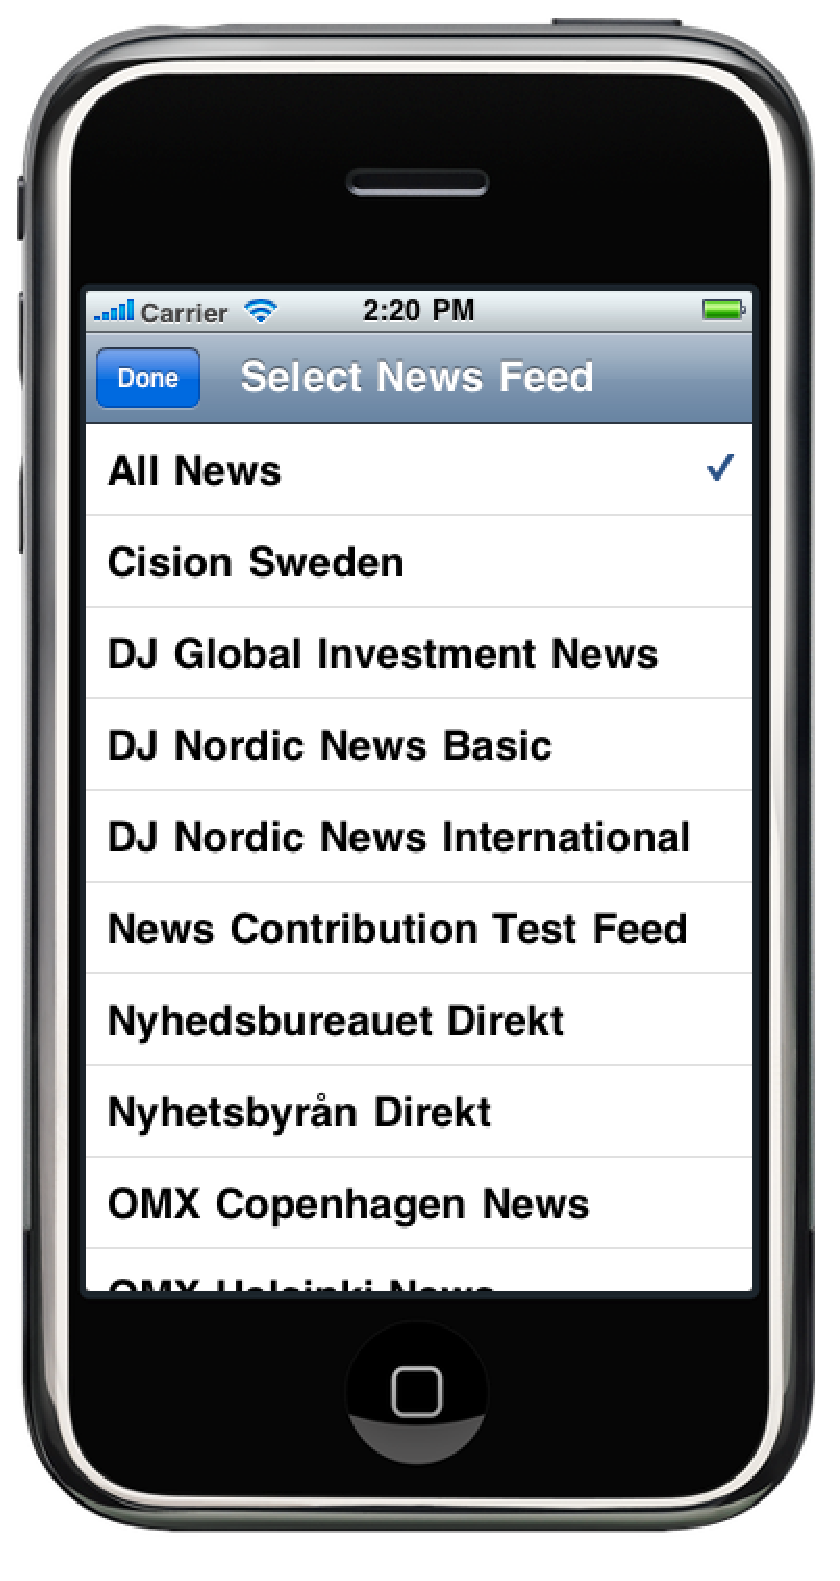
\includegraphics[scale=0.5]{newsFeedSelection}

News feed selection should be remembered after selection and be persistent between program launches and tab switching. After switching to a specific news feed you should see only news from that feed.

\section*{Settings Tab}
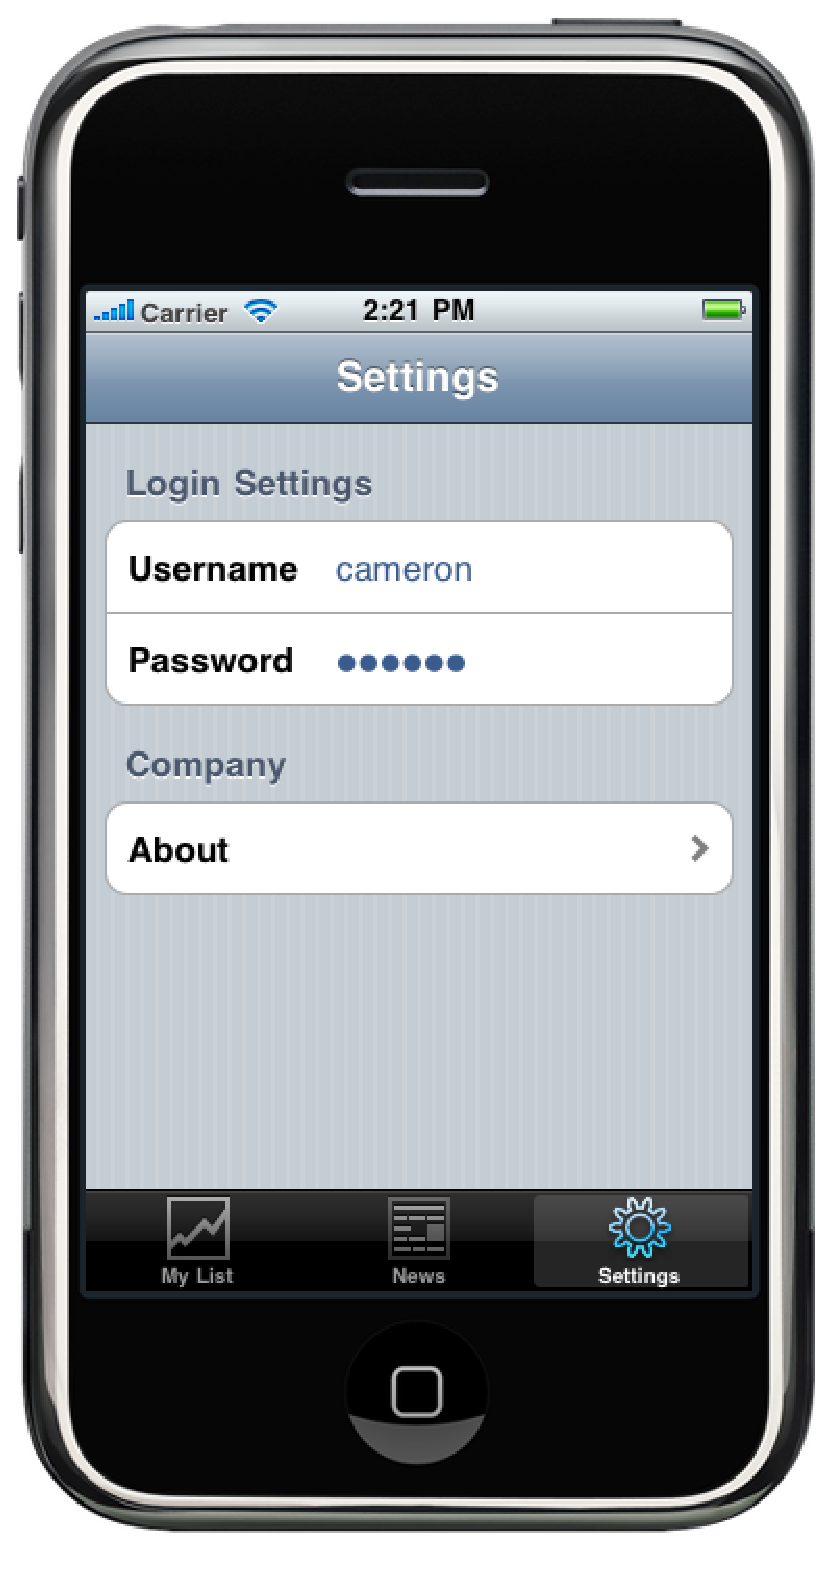
\includegraphics[scale=0.5]{settings}

Not having a username or password should result in a disconnection and during launch the user should be prompted to enter valid login details. Whenever the user enters valid details they should be logged in.

\end{document}